\subsection{Oreo}\label{cap:oreo}
\emph{Oreo} consiste in un programma che offe un servizio per la vendita di fucili. Le operazioni disponibili sono:
\begin{enumerate}
	\item \emph{Add new rifle}: dato un nome ed una descrizione, aggiunge in una lista, \verb+rifles+, il fucile da comprare. La vulnerabilità è presente proprio in questa operazione, poichè nella \verb+struct rifle_t+, vedi Listing~\ref{code:structrifle}, quando si inserisce o la descrizione o il nome si può fare un overflow sul campo \verb+next+
	\item \emph{Show added rifles}: mostra i fucili aggiunti in lista
	\item \emph{Order selected rifles}: ordina i fucili, facendo una \verb+free+ dei nodi della lista
	\item \emph{Leave a Message with your Order}: lascia un messaggio, scrivendo in un buffer contenuto in \verb+.bss+
	\item \emph{Show current stats}: mostra il numero di fucili comprati e, se presente, il messaggio lasciato con la precedente operazione.
\end{enumerate}

\begin{lstlisting}[style=CStyle, label={code:structrifle}, caption={\texttt{struct rifle\_t} contenuta in \emph{oreo}}]
struct rifle_t {
	char description[25];
	char name[27];
	struct rifle_t* next;
};
\end{lstlisting}

Un \verb+checksec+ sul binario, mostra che il file è compilato a 32 bit e che essendo non RELRO, è possibile scrivere nella \verb+.got+ e ha anche PIE disabilitato.

\begin{Verbatim}[commandchars=\\\{\}]
    Arch:     i386-32-little
    RELRO:    \textcolor{red}{No RELRO}
    Stack:    \textcolor{green}{Canary found}
    NX:       \textcolor{green}{NX enabled}
    PIE:      \textcolor{red}{No PIE (0x8048000)}
\end{Verbatim}

Ciò che è importante sapere ai fini dell'exploit è che tutte le strutture dati sono contenute nel segmento \verb+.bss+. In particolare esiste un puntatore ad un buffer di caratteri, denominato \verb+msg_ptr+, e il buffer puntato, denominato \verb+buf_msg+ di dimensione 0x80. \verb+msg_ptr+ è inizializzato nel \verb+main+ per puntare all'indirizzo di \verb+buf_msg+.
Inoltre ogni volta che viene aggiunto un nuovo fucile con l'operazione 1, viene allocato spazio in heap con una \verb+malloc+ e viene aggiunto in testa alla lista \verb+rifles+, prima che venga chiesto nome e descrizione.
Esiste infine un contatore, denominato \verb+cont+, che contiene il numero di fucili da ordinare, incrementato ogni volta che si esegue l'operazione 1, ma mai decrementato.

L'attacco utilizzato nell'exploit è denominato \emph{house of spirit}, in cui è possibile forzare la \verb+malloc + ad allocare uno spazio in memoria in un indirizzo arbitrario.
In questo caso è stato scelto come indirizzo una entry della tabella \verb+.got+, in modo da sovrascrivere il riferimento ad una funzione presente nella tabella stessa.

\begin{figure}
	\centering
	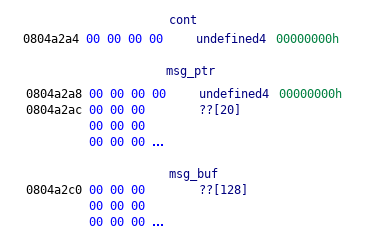
\includegraphics[width=8cm]{oreo-bss}
	\caption{Disposizione in \texttt{.bss} delle variabili globali}
	\label{fig:oreo-bss}
\end{figure}

In memoria, nel segmento \verb+.bss+, il contatore \verb+cont+ precede \verb+msg_ptr+, dopo di che seguono 20 byte inutilizzati, per poi esserci il buffer \verb+buf_msg+, secondo la Figura~\ref{fig:oreo-bss}.
Bisogna tener presente che per far credere alla \verb+free+ che l'attuale chunk da liberare è effettivamente un chuck e che questo deve andare in un fastbin, il campo \verb+size+ deve contenere una dimensione corretta, senza badare al bit \verb+prev_in_use+, che nella gestione di un fast bin non viene considerato.
Inoltre, poichè la \verb+malloc+ viene chiamata solo nell'operazione 1 e questa alloca uno spazio in memoria di 0x38 byte, serve un chunk di dimensione 0x40.
Il target scelto per la \verb+malloc+ è l'indirizzo di \verb+msg_ptr+, in modo tale da modificare il puntatore ad un buffer arbitrario, che è possibile poi sovrascrivere con l'operazione 4.

Quindi il campo \verb+size+ del chunk dato alla \verb+free+\footnote{ovvero i 4 byte precedenti al puntatore dato} deve contenere 0x40. Questo corrisponde in memoria alla variabile \verb+cont+, che è possibile incrementare solamente con l'operazione 1.

\begin{lstlisting}[style=PyStyle]
msg_ptr_addr = 0x0804a2a8

for i in range(0x40-1):
	add_rifle("a", "a")

payload = p8(0x61) * 27
payload += p32(msg_ptr_addr)

add_rifle(payload, "description")
\end{lstlisting}

Vengono inizialmente inserite in lista 0x40-1 fucili, per poi aggiungere un fucile, che tramite l'inserimento del nome\footnote{un campo di 27 byte}, sovrascrive il campo \verb+next+ con l'indirizzo di \verb+msg_ptr+.

Poichè la free controlla che il chunk successivo abbia una \verb+size+ maggiore di 16 e minore di 128k, dopo 36 byte in \verb+msg_buf+ viene scritto il valore 0x1234, che rientra nella size corretta:

\begin{lstlisting}[style=PyStyle]
payload = p8(0) * 36
payload += p32(0x1234)

leave_notice(payload)
\end{lstlisting}

Per fare in modo che il chunk iniettato sia il primo del fastbin, l'attraversamento della lista \verb+rifles+ deve terminare al chunk iniettato. Ecco il perchè del riempimento di \verb+msg_buffer+ con byte posti a 0.

La seguente istruzione farà finire \verb+msg_ptr_addr - 0x8+ nel fastbin\footnote{0x8 perchè il campo \verb+size+ e \verb+prev_size+ a 32 bit sono di 4 byte}.
Da notare inoltre l'allineamento del chunk a 16 byte, fornito alla free\footnote{si ricorda che il chunk address si ottiene dall'indirizzo fornito alla \verb+free+, a cui si sottrae l'header del chunk, in questo caso 8 byte}:

\begin{lstlisting}[style=PyStyle]
order()
\end{lstlisting}

\paragraph{Leak della libc e ottenimento della shell}
Si sovrascrive quindi \verb+msg_ptr+ con l'indirizzo della \verb+.got+ di \verb+strlen+:

\begin{lstlisting}[style=PyStyle]
add_rifle("name", p32(e.got['strlen']))     # overwrite msg_ptr with strlen got address

stats()

p.recvuntil("Order Message: ")
libc_addr = u32(p.recvline()[:4]) - 0x7e440
\end{lstlisting}

Con \verb+stats+, che corrisponde all'operazione 5, si stampa il contenuto del "\verb+msg_buf+", in questo caso il contenuto della \verb+.got+ di \verb+strlen+. Si ha quindi un leak della libc, ottenuto togliendo l'offset 0x7e440 all'indirizzo nella libc di \verb+strlen+.

Con il tool \verb+magic.py+\cite{magicpy}, si trova il \emph{magic gadget} che consente di eseguire \verb+exec("/bin/sh")+ con un solo gadget, per cui si sovrascrive il nuovo "\verb+msg_buf+" che corrisponde all'indirizzo della \verb+.got+ di \verb+strlen+ con il magic gadget:

\begin{lstlisting}[style=PyStyle]
leave_notice(p32(libc_addr + 0x5fbc5))      # magic gadget
\end{lstlisting}

Poichè l'operazione \verb+leave_notice+, operazione 4, dopo aver letto il messaggio da stdin determina la lunghezza della stringa inserita con \verb+strlen+, viene eseguito il gadget iniettato.
Si ottiene in questo modo una shell.